\section{Latent Planning Performance} \label{sec:exp_control}
\subsection{Planning evaluation setup}

\begin{figure}[t]
    \centering
    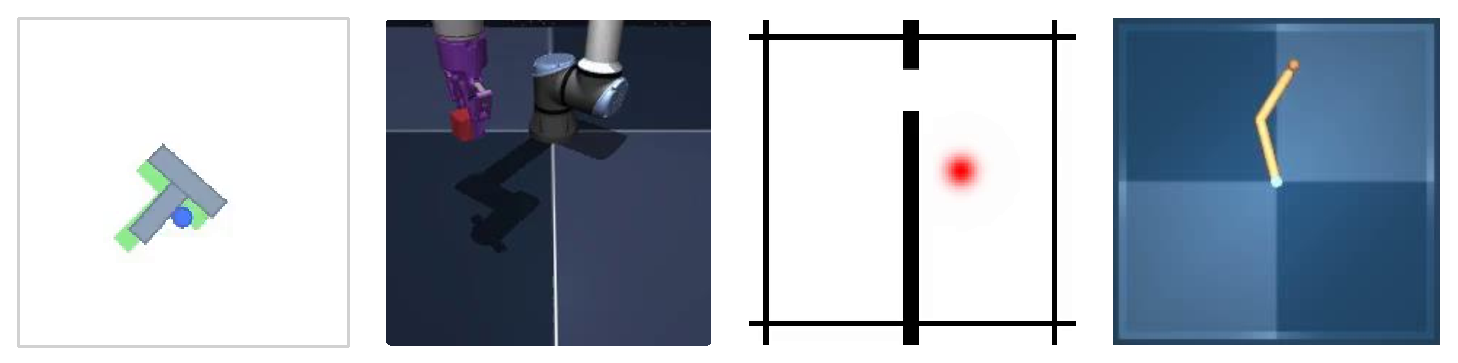
\includegraphics[width=\linewidth]{figs/envs.pdf}
    \caption{\small Environments used for evaluation. \textbf{Left:} Push-T, a 2D manipulation task where the agent must push a block toward a target configuration, commonly used as a robotics benchmark. \textbf{Center (1):} OGBench-Cube, a visually richer 3D manipulation environment where a robotic arm interacts with a cube to reach a target position. \textbf{Center (2):} Two-Room, a simple 2D navigation environment where an agent moves between rooms to reach target positions. \textbf{Right:} Reacher, a task where a 2-joint arm needs to reach a target configuration in a 2D plane. All environments have a continuous action space. More details on environment and datasets are available in appendix~\ref{appendix:envs}.}
    \label{fig:envs}
\end{figure}

\paragraph{Environments.}  We evaluate LeWM on a diverse set of tasks, including navigation, motion planning and manipulation, in both two- and three-dimensional environments, all illustrated in Fig.~\ref{fig:envs}. We provide more details on dataset generation and environments in App.~\ref{appendix:envs}.

\paragraph{Baselines.}  We compare the performance of LeWM against several baselines: DINO-WM and PLDM, two state-of-the-art JEPA-based methods; a goal-conditioned behavioral cloning policy (GCBC); and two goal-conditioned offline reinforcement learning algorithms, GCIVL and GCIQL.
Among these baselines, PLDM is the closest to our setup, as it also learns a world model end-to-end directly from pixel observations. However, it relies on a seven-term training objective derived from the VICReg criterion, which introduces training instability and increases the complexity of hyperparameter tuning. DINO-WM, in contrast, models dynamics using DINOv2~\cite{oquab2024dinov} as feature encoder to mitigate representation collapse, but its original formulation additionally incorporates other modalities, such as proprioceptive inputs; for a fair comparison, unless specified otherwise, we exclude proprioceptive information from DINO-WM. Additional implementation details for the baselines (App.~\ref{appendix:baselines}) and evaluation settings (App.~\ref{appendix:control_details}) are provided in the appendix. For each method, we keep the hyperparameters fixed across all environments.


\subsection{Towards Efficient Planning with WMs}


We report planning performance in Fig.~\ref{fig:ctrl-all}. LeWM improves over PLDM on the more challenging planning tasks, achieving an 18\% higher success rate on PushT while remaining competitive with DINO-WM. Notably, on PushT, LeWM (pixels-only) surpasses DINO-WM, even when DINO-WM has access to additional proprioceptive information, demonstrating LeWM’s ability to capture underlying task-relevant quantities. Moreover, when comparing planning speedups (Fig.~\ref{fig:planning-time}), LeWM achieves a 48× faster planning time, with the full planning completing in under one second while preserving competitive performance across tasks. This planning time is consistent across environments for a fixed planning setup, narrowing gap with real-time control.

We report planning performance in Fig.~\ref{fig:ctrl-all}. LeWM outperforms PLDM on the more challenging planning tasks, achieving an 18\% higher success rate on PushT, while remaining competitive with DINO-WM. Notably, on PushT, LeWM (pixels-only) surpasses DINO-WM even when DINO-WM has access to additional proprioceptive information, demonstrating LeWM’s ability to capture underlying task-relevant quantities. Interestingly, LeWM performs worse on the simplest environment, Two-Room. A possible explanation is that the low diversity and low intrinsic dimensionality of this dataset make it difficult for the encoder to match the isotropic Gaussian prior enforced by SIGReg in a high-dimensional latent space, which may lead to a less structured latent representation. This highlights a potential limitation of the SIGReg regularization in very low-complexity environments.

Moreover, when comparing planning speedups (Fig.~\ref{fig:planning-time}), LeWM achieves a $48\times$ faster planning time, with the full planning completing in under one second while preserving competitive performance across tasks. This planning time remains consistent across environments for a fixed planning setup, narrowing the gap toward real-time control.

\subsection{Towards Stable Training of World Models}

\paragraph{Ablations.} We perform ablations on several design choices of LeWM. First, we analyze the sensitivity of SIGReg to its internal parameters, namely the number of random projections and the number of integration knots. The performance is largely unaffected by these quantities, indicating that they do not require careful tuning. As a result, the regularization weight $\lambda$ remains the only effective hyperparameter. Since only a single hyperparameter needs to be tuned, grid search can be performed efficiently using a simple bisection strategy ($\mathcal{O}(\log n)$), whereas PLDM requires search in polynomial time ($\mathcal{O}(n^6)$). We also study the effect of the embedding dimensionality. While the representation dimension must be sufficiently large for the method to perform well, performance quickly saturates beyond a certain threshold, suggesting that the approach is robust to the precise choice of encoder capacity. Additionally, we examine the impact of the encoder architecture by replacing the default ViT encoder with a ResNet-18 backbone (Tab.~\ref{tab:encoder-arch}). LeWM achieves competitive performance with both architectures, indicating that it is largely agnostic to the choice of vision encoder. Details on all ablations are available in App.~\ref{appendix:ablations}.


\paragraph{Training Curves.}We report the training loss curves on PushT for LeWM in Fig.~\ref{fig:lewm-loss} and PLDM in Fig.~\ref{fig:pldm-loss}. The two-term objective of LeWM exhibits smooth and monotonic convergence: the prediction loss decreases steadily while the SIGReg regularization term drops sharply in the early phase of training before plateauing, indicating that the latent distribution quickly approaches the isotropic Gaussian target. In contrast, PLDM's seven-term objective displays noisy and non-monotonic behavior across several of its loss components. These observations highlight a key advantage of LeWM: by reducing the training objective to only two well-behaved terms, the training becomes significantly more stable, removing the need to balance competing gradients from multiple regularizers.

\begin{figure}[t]
    \centering
    
    \begin{subfigure}{0.24\linewidth}
        \centering
        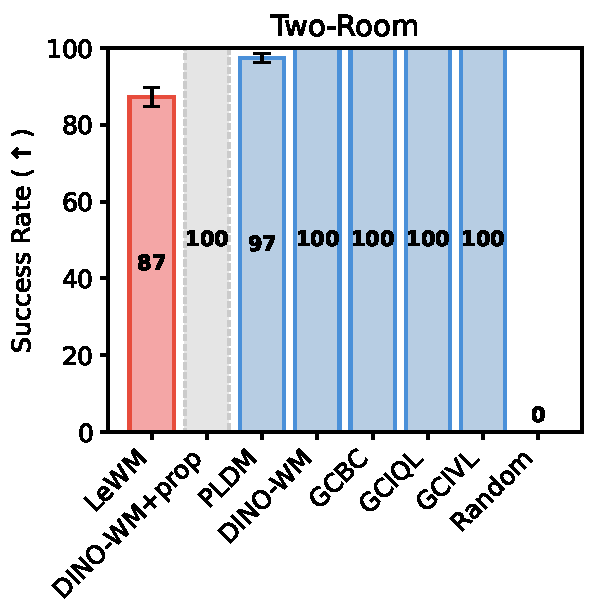
\includegraphics[width=\linewidth]{figs/ctrl-two-room.pdf}
    \end{subfigure}
    \hfill
    \begin{subfigure}{0.24\linewidth}
        \centering
        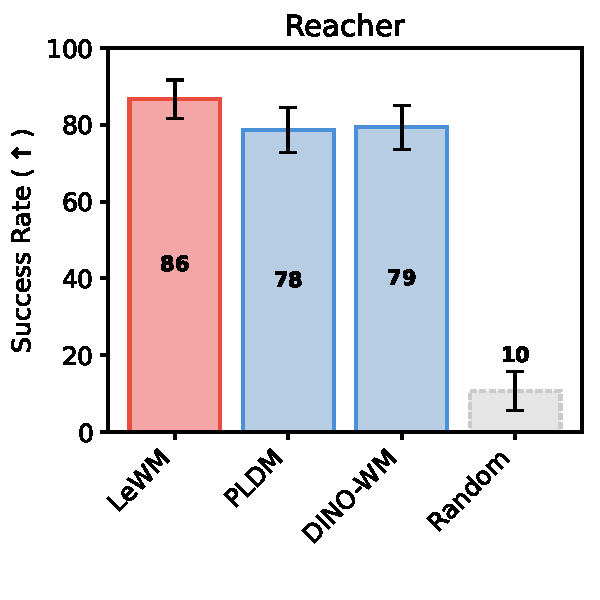
\includegraphics[width=\linewidth]{figs/ctrl-reacher.pdf}
    \end{subfigure}
    \hfill
    \begin{subfigure}{0.24\linewidth}
        \centering
        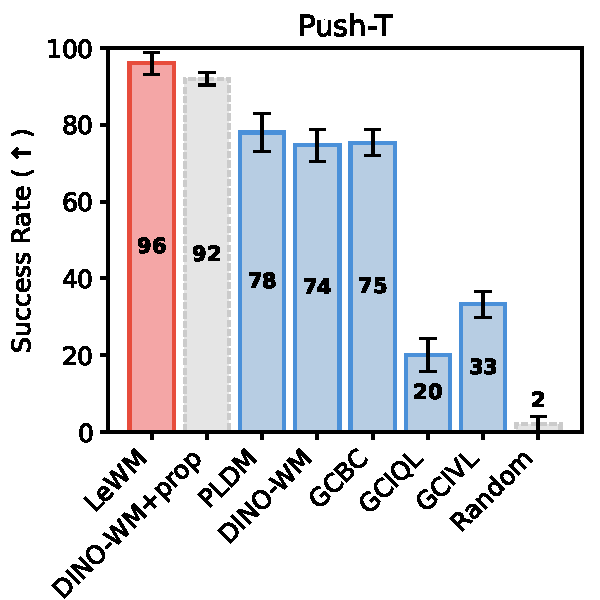
\includegraphics[width=\linewidth]{figs/ctrl-push-t.pdf}
    \end{subfigure}
    \hfill
    \begin{subfigure}{0.24\linewidth}
        \centering
        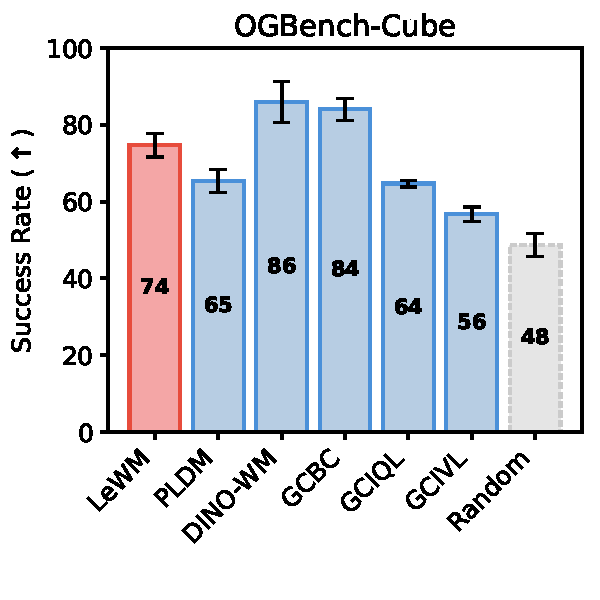
\includegraphics[width=\linewidth]{figs/ctrl-ogbench-cube.pdf}
    \end{subfigure}

    \caption{\small \textbf{Planning performance across environments.} 
    Results are shown for \textit{Two-Room} (left), \textit{Reacher} (center 1), \textit{PushT} (center-2) and \textit{OGBench-Cube} (right). 
    LeWM consistently outperforms PLDM and DINO-WM on Push-T and Reacher. On OGBench-Cube, DINO-WM slightly outperforms LeWM, possibly due to the higher visual complexity and the 3D nature of the environment, which makes encoder training more challenging. In the simpler Two-Room environment, PLDM and DINO-WM outperform LeWM, which may be explained by the SIGReg regularization encouraging a Gaussian distribution in a high-dimensional latent space, while the intrinsic dimensionality of the environment is much lower.}
    \label{fig:ctrl-all}
\end{figure}


\section{Quantifying Physical Understanding in LeWM}


In this section, we evaluate the quality of the dynamics captured by LeWM’s latent space, either by learning to extract physical quantities from latent embeddings or by measuring the world model’s ability to detect changes in physics.

\subsection{Physical Structure of the Latent Space}

\paragraph{Probing physical quantities.} As a first measure of physical understanding, we evaluate which physical quantities are recoverable from LeWM’s latent representations. We train both linear and non-linear probes to predict physical quantities of interest from a given embedding. Results on the Push-T environment are reported in Tab.~\ref{tab:probe-pusht}. Our method consistently outperforms PLDM while remaining competitive with representations produced by large pretrained models such as DINOv2. We provide probing results on other environments in App.~\ref{appendix:probing}.

\begin{table}[h]
\centering
\caption{\small \textbf{Physical latent probing results on Push-T.} LeWM consistently
outperforms PLDM while remaining competitive with DINO-WM. The strong probing
performance of DINO-WM on certain properties may stem from its foundation-model
pretraining: the DINOv2 encoder is trained on two orders of magnitude more data
($\sim$124M images) spanning a far more diverse
distribution, which likely allows it to capture some physical properties in its
embeddings by default.}
\resizebox{\textwidth}{!}{%
\begin{tabular}{l l c c c c}
\toprule
& & \multicolumn{2}{c}{\textbf{Linear}} & \multicolumn{2}{c}{\textbf{MLP}}\\
\cmidrule(lr){3-4} \cmidrule(lr){5-6}
\textbf{Property} & \textbf{Model} & MSE $\downarrow$ & r $\uparrow$ & MSE $\downarrow$ & r $\uparrow$\\
\toprule
\multirow{3}{*}{Agent Location}
  & DINO-WM & $1.888 \pm 0.500$ & $\mathbf{0.977}$ & $\mathbf{0.003 \pm 0.022}$ & $\mathbf{0.999}$\\
  & PLDM    & $0.090 \pm 0.311$ & $0.955$ & $0.014 \pm 0.119$ & $0.993$\\
  & LeWM    & $\mathbf{0.052 \pm 0.149}$ & $0.974$ & $0.004 \pm 0.056$ & $0.998$\\
\midrule
\multirow{3}{*}{Block Location}
  & DINO-WM & $\mathbf{0.006 \pm 0.007}$ & $\mathbf{0.997}$ & $0.002 \pm 0.003$ & $\mathbf{0.999}$\\
  & PLDM    & $0.122 \pm 0.341$ & $0.938$ & $0.011 \pm 0.066$ & $0.994$\\
  & LeWM    & $0.029 \pm 0.073$ & $0.986$ & $\mathbf{0.001 \pm 0.006}$ & $\mathbf{0.999}$\\
\midrule
\multirow{3}{*}{Block Angle}
  & DINO-WM & $\mathbf{0.050 \pm 0.101}$ & $\mathbf{0.979}$ & $\mathbf{0.009 \pm 0.052}$ & $\mathbf{0.995}$\\
  & PLDM    & $0.446 \pm 0.625$ & $0.745$ & $0.056 \pm 0.184$ & $0.972$\\
  & LeWM    & $0.187 \pm 0.359$ & $0.902$ & $0.021 \pm 0.139$ & $0.990$\\
\bottomrule
\end{tabular}%
}
\vspace{2mm}
\label{tab:probe-pusht}
\end{table}

\begin{figure}[t]
    \centering
    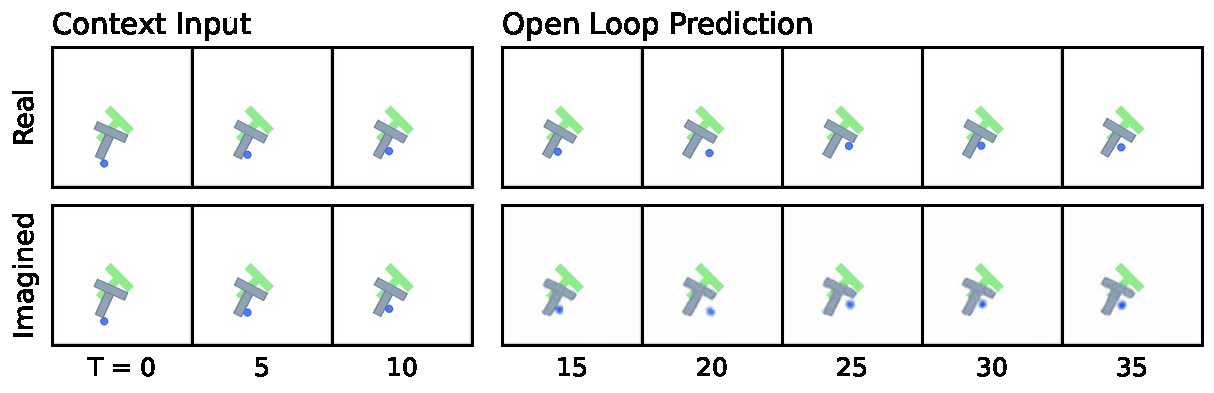
\includegraphics[width=\linewidth]{figs/pusht_rollout.pdf}\\
    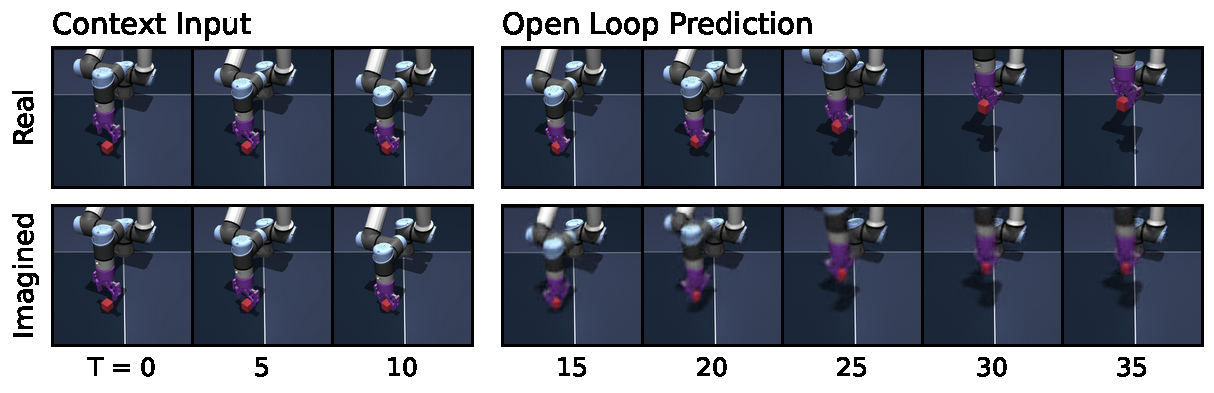
\includegraphics[width=\linewidth]{figs/cube_rollout.pdf}
    \caption{\textbf{Predictor rollouts on PushT and OGBench-Cube.} 
    We visualize decoded latent plans produced by LeWM given a context and an action sequence. Each rollout uses three image observations as context, which are encoded into latent representations. Conditioned on the action sequence, the predictor autoregressively generates future latent states in an open-loop manner. All predicted latents are decoded into images using a decoder that was not used during training. The resulting imagined rollouts closely match the real observations, demonstrating that the latent representation effectively captures the overall scene structure and essential environment dynamics. Some finer details, however, are not fully captured by LeWM; for instance, the angle of the end-effector in OGBench-Cube. Additional rollouts are provided in Fig.~\ref{fig:rollout-2}.}
    \label{fig:rollout}
\end{figure}

\begin{figure}[h]
    \centering
    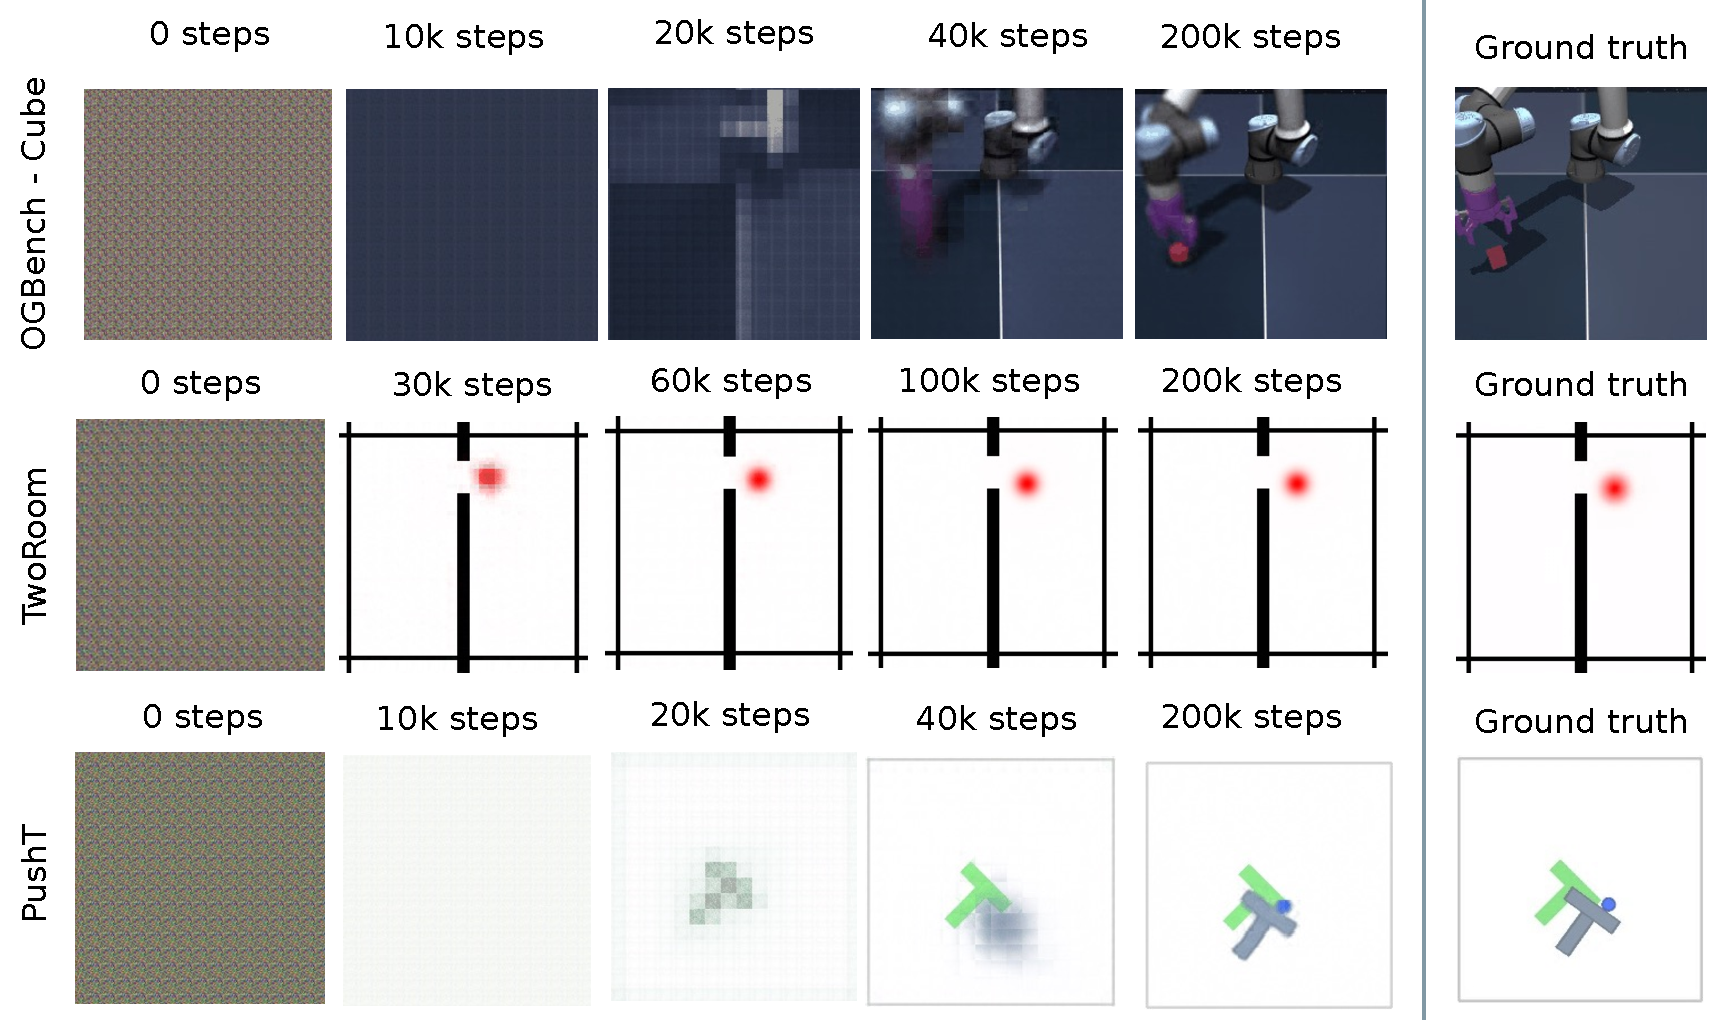
\includegraphics[width=\linewidth]{figs/decoder_training.pdf}
    \caption{\small \textbf{Decoder visualization during training.} As training progresses, the latent representation increasingly captures the information required to reconstruct the visual scene, even though no reconstruction loss is used during training. Early in training, the decoded images correspond to slow features, a phenomenon previously reported~\cite{sobal2022jointembeddingpredictivearchitectures}.}
    \label{fig:decoder-vis}
\end{figure}


\begin{figure}
    \centering
    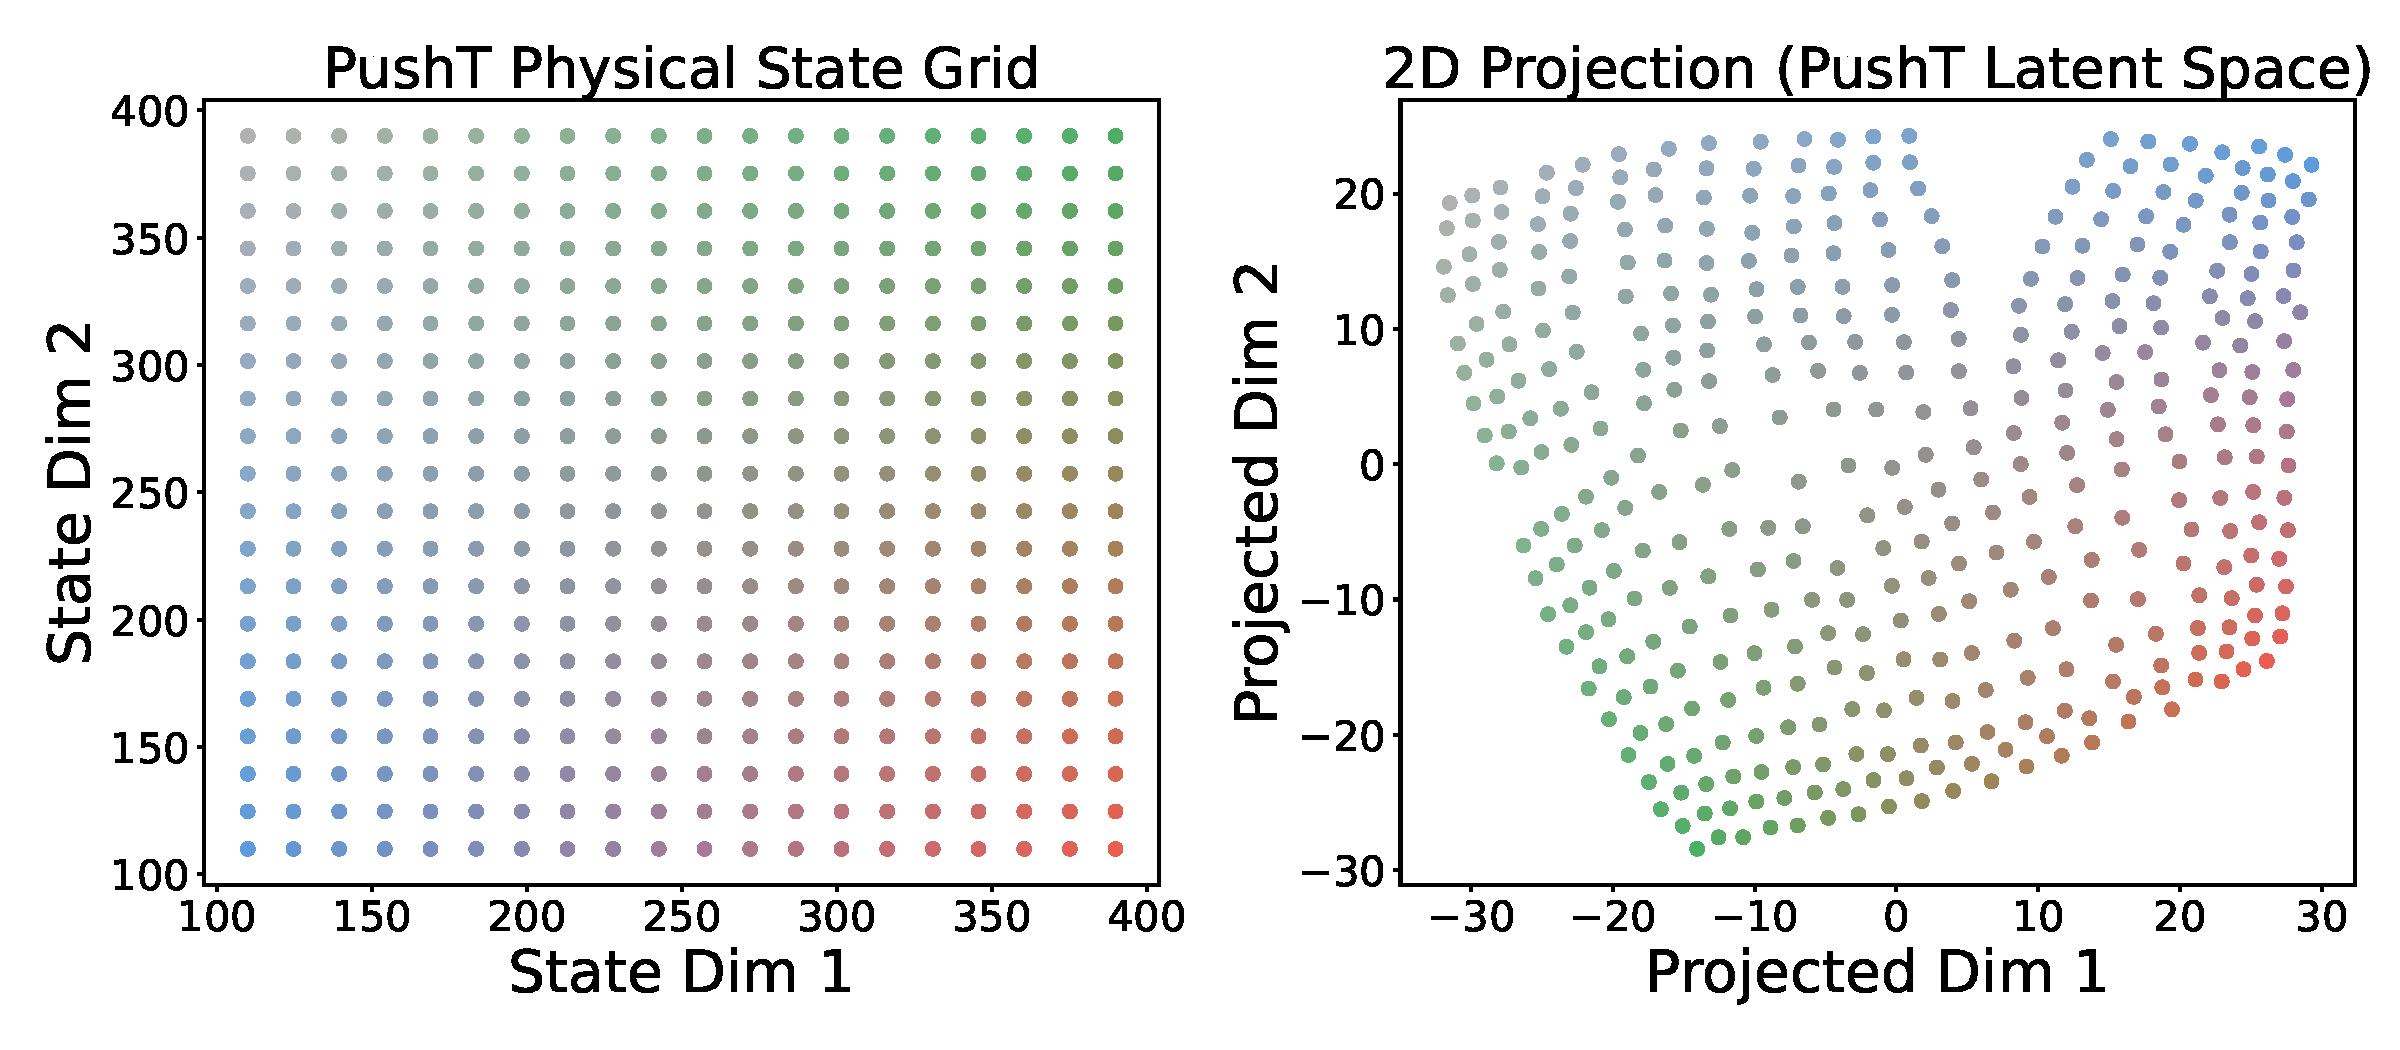
\includegraphics[width=\linewidth]{figs/pusht_lejepa_epoch_10_tsne.pdf}
    \caption{\small \textbf{Visualization of the latent space}  obtained with LeWM for the PushT environment. On the left, the grid of states is obtained by moving the agent and the block in the x-y plane. On the right, the embeddings of these states are visualized using a t-SNE.}
    \label{fig:tsne_pusht_lejepa}
\end{figure}

\paragraph{Decoding Latent Space.}
To further assess the information captured in the latent representation, we report in Fig.~\ref{fig:decoder-vis} images produced by a decoder trained to reconstruct pixel observations from a single latent embedding (192 dim) during training. Although reconstruction is never used during training, the decoder is able to recover the visual scene from the learned representation, confirming that the low-dimensional and compact latent space retains sufficient information about the underlying physical state. Details on the decoder architecture are provided in App.~\ref{appendix:details}.

\paragraph{Visualizing Latent Space.} We further visualize the structure of the latent space using t-SNE. Fig.~\ref{fig:tsne_pusht_lejepa} provides a qualitative visualization of the latent space in the \textit{PushT} environment. The visualization suggests that the learned representation captures the spatial structure of the environment, preserving neighborhood relationships and relative positions in the latent space.

\paragraph{Temporal Latent Path Straightening.} Inspired by the temporal straightening hypothesis from neuroscience \citep{henaff2019perceptual}, we measure the cosine similarity between consecutive latent velocity vectors throughout training (Eq.~\ref{eq:path-straightening}). We find that LeWM's latent trajectories become increasingly straight on PushT over training as a purely emergent phenomenon, without any explicit regularization encouraging this behavior, cf. Fig.~\ref{fig:tmp-straight}. Remarkably, LeWM achieves higher temporal straightness than PLDM, despite PLDM employing a dedicated temporal smoothness regularization term. We detail our findings in App.~\ref{appendix:tmp-straight}.

\subsection{Violation-of-expectation Framework} \label{subsec:voe}

\begin{figure}
    \centering
    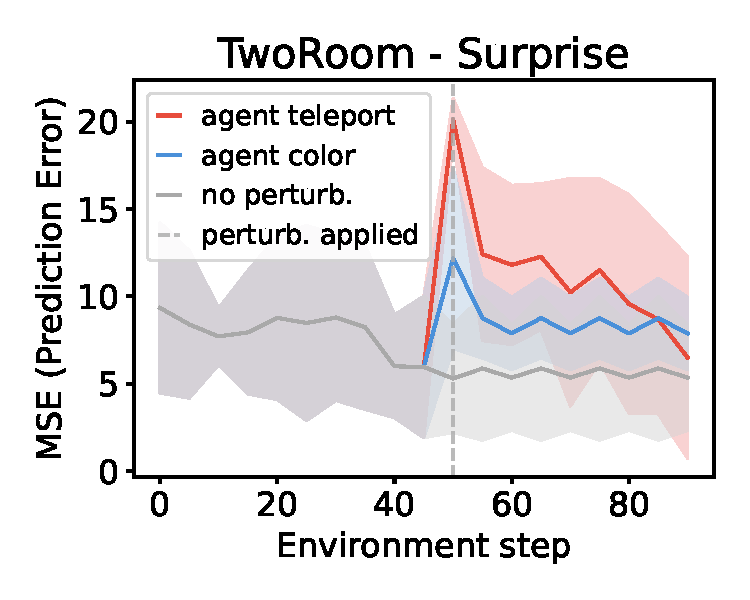
\includegraphics[width=0.32\linewidth]{figs/surprise_tworoom_lejepa_epoch_80.pdf}
    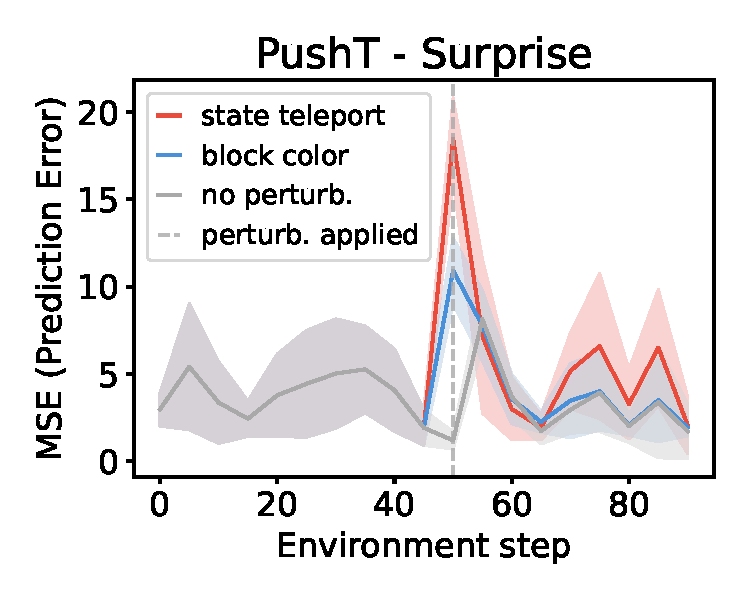
\includegraphics[width=0.32\linewidth]{figs/surprise_pusht_lejepa_epoch_10.pdf}
    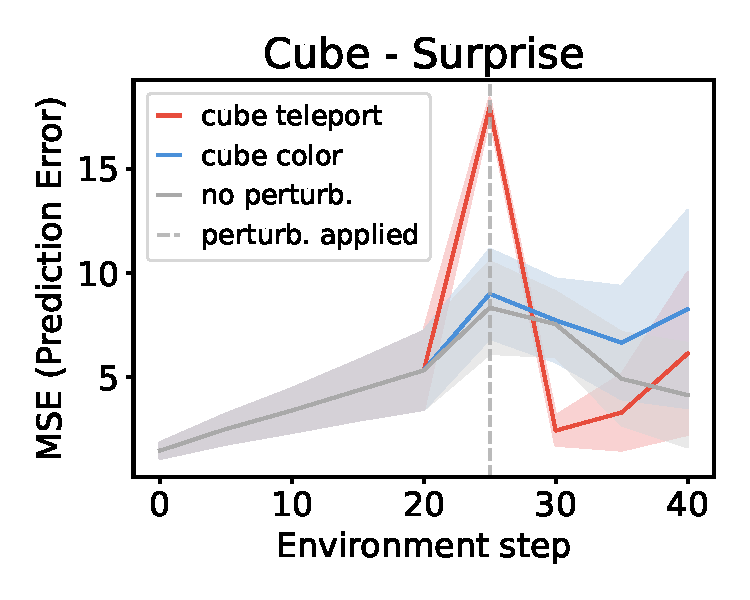
\includegraphics[width=0.32\linewidth]{figs/surprise_cube_lejepa_epoch_10.pdf}
    \caption{\textbf{Violation-of-expectation evaluation across three environments.} Each plot shows the model's surprise along three trajectories: an unperturbed reference trajectory, a visually perturbed trajectory where an object's color changes abruptly, and a physically perturbed trajectory where one or more objects are teleported to a random position. The teleportation violates physical continuity and produces a pronounced spike in surprise, while the unperturbed trajectory maintains a low baseline. Surprise is significantly higher for teleportation perturbations across all three environments (paired t-test, $p<0.01$), whereas for the cube color perturbation the increase is weaker and not significant, indicating that the model is more sensitive to physical perturbations than to visual ones. From left to right, the environments are \textit{TwoRoom}, \textit{PushT}, and \textit{OGBench Cube}.}
    \label{fig:voe_surprise_lejepa}
\end{figure}


Another approach to quantifying physical understanding is the ability to detect violations of the learned world model. Inspired by the violation-of-expectation (VoE) paradigm used in developmental psychology and recently adopted in machine learning \cite{margoni2024violation, garrido2025intuitive, bordes2025intphys2}, this framework evaluates whether a model assigns higher surprise to events that contradict learned physical regularities.


Following prior work, we quantify surprise by measuring the discrepancy between the model’s predicted future observations and the actual observed future. We evaluate this framework across three environments: \textit{TwoRoom}, \textit{PushT}, and \textit{OGBench Cube}. For each environment, we introduce two types of perturbations. The first is a visual perturbation, where the color of an object changes abruptly during the trajectory. The second is a physical perturbation, where one or more objects are teleported to a random location, violating the expected physical continuity of the scene.  Fig.~\ref{fig:voe_surprise_lejepa} shows that LeWM consistently assigns higher surprise to frames containing physical violations compared to their unperturbed counterparts. We provide more details on VoE in App.~\ref{appendix:voe}.
